%-----------------------------------------------
% Template para criação de resumos de projectos/dissertação
% jlopes AT fe.up.pt,   Fri Jul  3 11:08:59 2009
%-----------------------------------------------

\documentclass[9pt,a4paper]{extarticle}

%% English version: comment first, uncomment second
\usepackage[portuguese]{babel}  % Portuguese
%\usepackage[english]{babel}     % English
\usepackage{graphicx}           % images .png or .pdf w/ pdflatex OR .eps w/ latex
\usepackage{times}              % use Times type-1 fonts
\usepackage[utf8]{inputenc}     % 8 bits using UTF-8
\usepackage{url}                % URLs
\usepackage{multicol}           % twocolumn, etc
\usepackage{float}              % improve figures & tables floating
\usepackage[tableposition=top]{caption} % captions
%% English version: comment first (maybe)
\usepackage{indentfirst}        % portuguese standard for paragraphs
%\usepackage{parskip}

%% page layout
\usepackage[a4paper,margin=30mm,noheadfoot]{geometry}

%% space between columns
\columnsep 12mm

%% headers & footers
\pagestyle{empty}

\graphicspath{{figures/}}

%% figure & table caption
\captionsetup{figurename=Fig.,tablename=Tab.,labelsep=endash,font=bf,skip=.5\baselineskip}

%% heading
\makeatletter
\renewcommand*{\@seccntformat}[1]{%
  \csname the#1\endcsname.\quad
}
\makeatother

%% avoid widows and orphans
\clubpenalty=300
\widowpenalty=300

\begin{document}

\title{\vspace*{-8mm}\textbf{\textsc{Social Media Text Processing and\\ Semantic Analysis for Smart Cities}}}
\author{\emph{João Filipe Figueiredo Pereira}\\[2mm]
\small{Projecto de Dissertação de Mestrado desenvolvido com a orientação do \emph{Prof.\ Rosaldo Rossetti} e \emph{Pedro Saleiro} no \emph{LIACC}}}
\date{}
\maketitle
%no page number 
\thispagestyle{empty}

\vspace*{-4mm}\noindent\rule{\textwidth}{0.4pt}\vspace*{4mm}

\begin{multicols}{2}

\section{Motivação}\label{sec:motivation}

%Neste documento apresentam-se alguns conselhos e instruções para a preparação dos resumos de projecto/dissertação. 
%Pede-se aos autores o favor de, dentro do possível, cumprirem com as instruções que são dadas, assim como com a estrutura apresentada, de forma a manter-se o mesmo aspecto em todos os resumos. 
%Nas sub-secções~\ref{sec:lingua} a ~\ref{sec:number} podem encontrar-se alguns detalhes sobre a formatação do documento. 

%Na secção ``Motivação'' deve ser apresentado o enquadramento do trabalho, dando ideia das necessidades que o mesmo cobre.

Devido à ascensão das Redes Sociais, as pessoas obtêm e partilham informação quase que instantaneamente 24/7. Muitas áreas de investigação tentaram extrair informações importantes destes grandes volumes de conteúdo, gerado por utilizadores, e livremente disponíveis. As áreas de investigação de sistemas inteligentes de transportes e de cidades inteligentes (\textit{smart cities}) não são excepção. Contudo, extrair conhecimento acionável e significativo de conteúdo gerado por utilizadores exige um esforço complexo. Primeiro, cada serviço de social media possui as suas próprias especificidades e restrições para o método de recolha dos dados; em segundo lugar, o volume de mensagens produzidas pode ser esmagador para o processamento automático e prospeção; e por último, não menos importante, os textos das redes sociais são, geralmente, curtos, informais, com muitas abreviações, jargões, gírias e expressões idiomáticas.

\section{Descrição do Problema}
Extrair conhecimento de dados do Twitter é um processo trabalhoso e demorado devido às restrições e dificuldades do conteúdo das mensagens. A informalidade, a existência de gírias, abreviaturas, jargões, e o curto comprimento das mensagens são alguns dos problemas emergidos durante  a análise deste tipo de dados. Recolher \emph{tweets} de forma automática e, ao mesmo tempo, extrair informação valiosa para cidades inteligentes e para a área de transportes torna a tarefa ainda mais complexa.  A absência de \emph{gold-standard datasets} é o problema mais perturbador, uma vez que não somos capazes de comparar as análises realizadas para as áreas de estudo acima mencionados.
O problema em foco nesta dissertação é encontrar uma forma de demonstrar análises de texto das redes sociais sobre cidades/regiões/países que possam ser valiosas para entidades, governos ou até cidadãos comuns em processos de tomada de decisão, como, por exemplo, qual a cidade com nível de segurança mais elevado, ou qual o melhor meio de transporte que um indivíduo pode escolher para viajar em uma cidade.

\section{Objectivos}\label{sec:goals}

%A secção ``Objectivos'' deve enunciar claramente os objectivos a atingir com o trabalho de projecto/dissertação, enquadrando-os na respectiva área de actividade a que o trabalho se destina. 
%Por exemplo, este documento tem como objectivos:
%\begin{itemize}
%\item Servir de modelo/exemplo do ponto de vista da dos resumos;
%\item Apresentar o aspecto gráfico que se pretende para os resumos;
%\item Disponibilizar \emph{templates} a quem pretenda utilizar \LaTeX.
%\end{itemize}

Foram estabelecidos nove objectivos diferentes nesta dissertação para atingirmos o nosso alvo principal:
\begin{itemize}
	\item Recolha contínua de \emph{tweets} georreferenciados de múltiplas \emph{bounding boxes} em paralelo e de acordo com os limites de utilização da \emph{API} do \emph{Twitter}
	\item Abordar as inconsistências e as filtragens de \emph{tweets} com ruído da \emph{API} \emph{Twitter Geo}
	\item Implementar métodos padrão de pré-processamento de texto para mensagens das redes sociais.
	\item Análise de conteúdo recorrendo a modelação de tópicos e caracterização comparativa entre diferentes \emph{bounding boxes} (por exemplo, cidades)
	\item Utilização de aprendizagem supervisionada na classificação de \emph{tweets} relacionados com viagens e transportes
	\item Treino de \emph{word embeddings} a partir de \emph{tweets} georreferenciados
	\item Estudar o impacto de \emph{word embeddings} em tarefas de classificação de \emph{tweets} relacionados com viagens e transportes 
	\item Criação de dados \emph{gold-standard} para aprendizagem supervisionada relacionada com viagens e transportes
	\item Agregação e visualização de resultados
\end{itemize}

\section{Proposta de Solução}\label{sec:work}

Nesta secção é descrito o problema a ser abordado nesta dissertação bem como a arquitectura e a implementação da framework por nós proposta para resolução do problema apresentado, assim como os seus principais módulos constituintes.

\begin{figure}[H]
\centerline{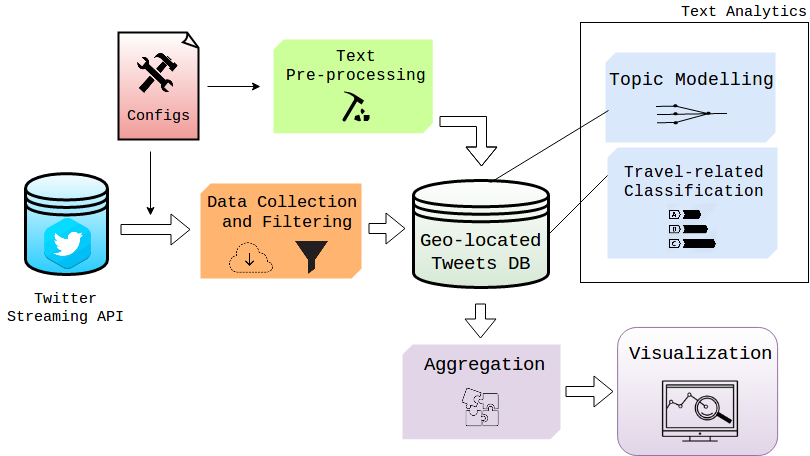
\includegraphics[scale=.25]{architecture.png}}
\caption{Visão geral da arquitectura da \emph{framework}}  
\label{fig:architecture}
\end{figure}

\subsection{Recolha e Filtragem de Dados}
O módulo de recolha de dados foi desenvolvido recorrendo a uma biblioteca \emph{open-source} de Python, conhecida como \emph{Tweepy}, que permite o acesso às \emph{APIs} do Twitter. Nós explorámos a \emph{Twitter Streaming API} usando heurísticas de localização, que permitem a recolha de \emph{tweets} georreferenciados através de uma sobreposição com \emph{bounding-boxes}.

\subsection{Pre-processamento de Texto}
Nós aplicamos um grupo considerável de operaões de pré-processamento de texto às mensagens tais como \emph{lowercasing}, \emph{lemmatization}, \emph{tokenization}, transformação de characters repetidos, filtragem de metadados, símbolos numéricos no texto e também remoção de palavras curtas e comuns.

\subsection{Modelação de Tópicos}
Redes sociais, mais especificamente, micro-blogs são serviços onde as pessoas publicam e partilham as suas opiniões e por esta razão são vistos como uma rica fonte de dados a explorar. De forma a explorar informação deste tipo de dados, nós implementámos na nossa \emph{framework} um módulo generativo utilizando técnicas de modelação de tópicos. Nós escolhemos o modelo \emph{Latent Dirichlet Allocation}~\cite{blei2003latent} para a implementação do módulo e realizamos testes em duas cidades Brazileiras, Rio de Janeiro e São Paulo, utilizando um total de 9.5M de tweets georreferenciados. No final, foram descobertos 29 tópicos latentes (Figure~\ref{fig:topics}) diferentes que caracterizam as duas cidades, sendo que 2 deles são únicos para cada cidade.

\begin{figure}[H]
	\centerline{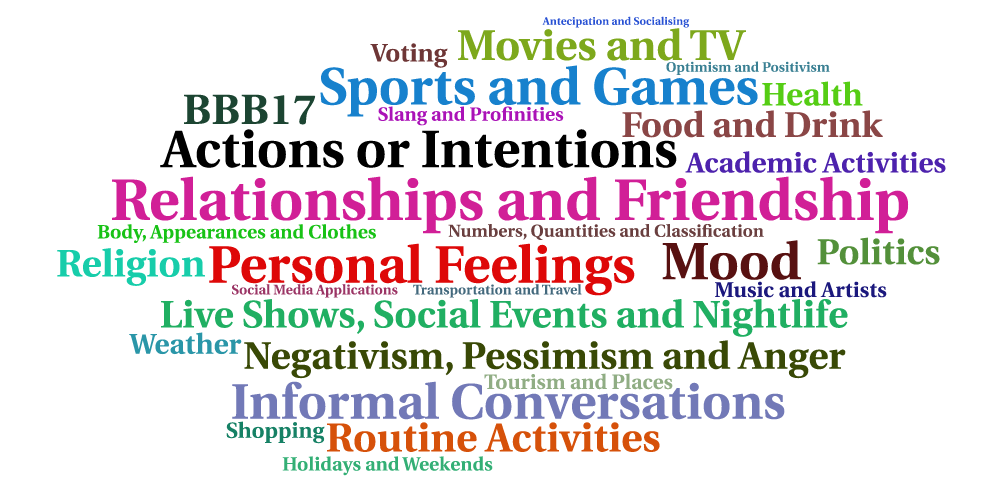
\includegraphics[scale=.16]{topics.png}}
	\caption{Tópicos latentes para as cidades do Rio de Janeiro e São Paulo}  
	\label{fig:topics}
\end{figure}

\subsection{Classificação de Tweets sobre Transportes}
Tentamos extrair e caracterizar tweets relacionados com viagens e transportes de grandes conjuntos de dados, a fim de estudar as distribuições geográficas e temporais deste conteúdo específico. As entidades de transporte poderão tirar proveito desse tipo de informação, uma vez que podem estudar os padrões de  mobilidade humana, bem como as opiniões dos cidadãos sobre determinados serviços de transporte. Realizamos experiências no Rio de Janeiro, São Paulo e Nova Iorque para discriminar tweets relacionados a viagens e transportes. Devido ao volume de dados recolhidos para cada cenário, foi necessário identificar automaticamente os tweets cujo conteúdo de alguma maneira sugere estar relacionado ao domínio de transportes. As abordagens convencionais exigem que especifiquemos palavras-chave relacionadas a viagens e transportes para classificar \emph{tweets}. Por outro lado, \emph{word embeddings}~\cite{mikolov2013linguistic} é uma forma de representação de texto que tenta capturar relações sintáticas e semânticas das palavras. O resultado é uma representação mais coesa onde palavras semelhantes são representadas por vectores semelhantes. Por exemplo, \emph{"taxi"/"uber"},\emph{"busão/ônibus"}, \emph{"ir para o trabalho"/"ir para a escola"} são casos em que os vetores produzidos são semelhantes. Foram estabelicidos diferentes grupos de \emph{features} para treinar os nossos classificares de texto, nomeadamente \emph{bag-of-words}, \emph{bag-of-embeddings} e ambos, combinando horizontalmente as suas matrizes de representação de texto.

\begin{figure}[H]
	\centerline{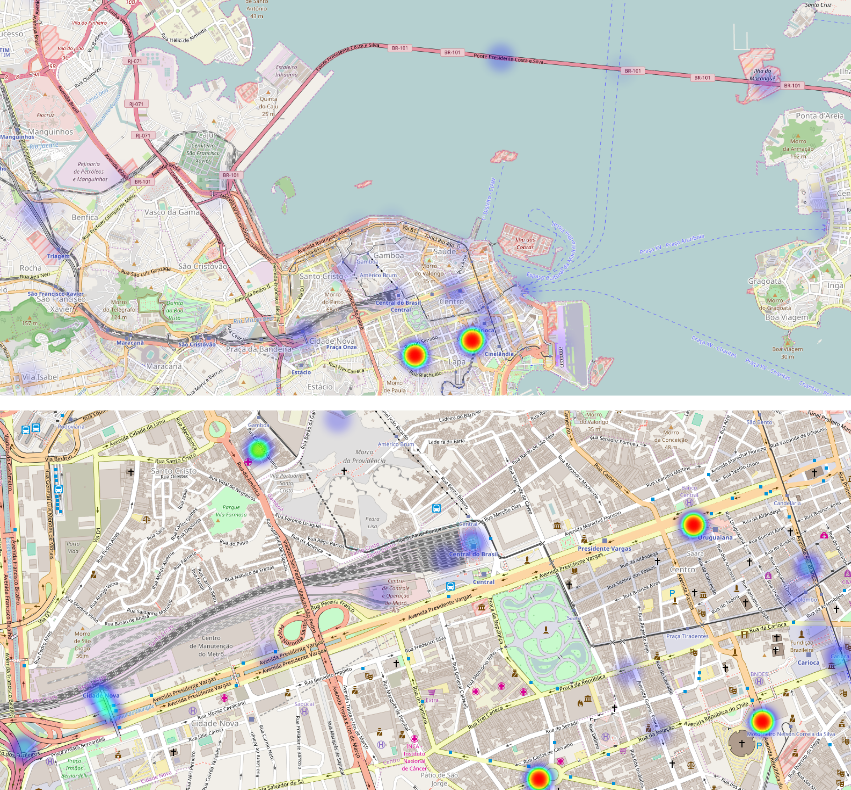
\includegraphics[scale=.18]{rio_tweets_transportation.png}}
	\caption{Aglomerações de \emph{tweets} classificados como relacionados com transportes na cidade do Rio de Janeiro}  
	\label{fig:rio_tweets_transportation}
\end{figure}
%Na secção ``Descrição do Trabalho'' (com este ou com outro nome que se julgue mais adequado) devem ser apresentadas as principais partes do trabalho, começando pela sua estruturação. Devem ser mencionadas as tecnologias utilizadas, com referências à sua interdependência e interligação dando especial ênfase aos componentes desenvolvidos pelo estudante no âmbito do trabalho em causa.

%No presente documento, seguem-se 9 subsecções com instruções acerca da extensão da comunicação, margens, estilos e outras recomendações gerais acerca da elaboração da versão final dos resumos.

%\subsection{Línguas Obrigatórias}\label{sec:lingua}

%Os resumos deverão ser apresentados, em ficheiros separados, em versões portuguesa e inglesa. 
%No resumo em Português e em caso de necessidade de utilização de termos em língua Inglesa, estes deverão ser devidamente salientados pela adopção da fonte em itálico, como, por exemplo, \emph{Ray-Tracing}.

%\subsection{Cabeçalho de Identificação}

%O cabeçalho de identificação deve ser centrado e inicia-se com o título da comunicação, em letras maiúsculas de tamanho 12 e em negrito. 
%Seguem-se, em linhas separadas e em tamanho 9, a identificação do estudante, da empresa e dos orientadores (estes dois numa única linha). 
%Todos os quatro nomes devem ser em itálico.

%\subsection{Extensão do Artigo e Tipo de Letra}

%Cada resumo deve ser formatado com texto a duas colunas, não devendo exceder duas páginas de formato A4. 
%\textbf{As duas colunas devem terminar sensivelmente à mesma altura}, em cada uma das páginas. 

%O tipo de letra para o texto genérico deverá ser \emph{Times New Roman} com tamanho 9 e espaçamento simples entre linhas. 
%O espaçamento entre parágrafos deverá ser estendido a 1.5 linhas (0.5 linha de espaçamento extra).

%\subsection{Dimensões das Margens}

%As margens a manter à volta do texto deverão ser as constantes na Tab.~\ref{tab:medidas}.

%\begin{table}[H]
%  \centering
%  \caption{Margens expressas em centímetros}
%\begin{tabular}{c | c}
%	\hline
%\textbf{Espaçamento} & \textbf{Medida}\\
%	\hline
%	\hline
%       Margem Superior & 3 cm\\
%       Margem Inferior & 3 cm\\
%        Margem Esquerda & 3 cm\\
%        Margem Direita  & 3 cm\\
%        Entre Colunas   & 1.2 cm\\
%	\hline
%\end{tabular}
%  \label{tab:medidas}
%\end{table}

%\subsection{Corpo do Texto}

%Todos os títulos de secções e subsecções devem ser escritos em negrito e com um espaçamento para cima ligeiramente superior ao de um parágrafo normal. 
%Os títulos de níveis um e dois devem ter tamanhos, respectivamente, 11 e 9. 
%As ``subsubsecções'' devem ser evitadas.

%\subsection{Numeração das Secções}

%As secções deverão ser numeradas com início em "1", de acordo com os níveis e subníveis respectivos, usando-se o ponto como separador.

%\subsection{Figuras, Equações e Quadros}

%As figuras e as tabelas deverão ser centradas, sempre que possível, à largura da coluna de texto em que se
%inserem (Tab.~\ref{tab:medidas} e Fig.~\ref{fig:figura}). 
%As figuras e tabelas cujas dimensões não o permitam, podem ser centradas à largura da página.

%\begin{figure}[H]
%\centerline{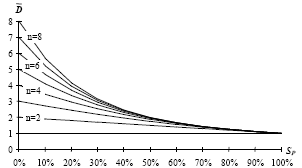
\includegraphics[scale=.6]{figura.png}}
%\caption{Esta é a legenda da figura}  
%\label{fig:figura}
%\end{figure}

%As legendas das figuras, a negrito, devem ser colocadas na sua parte inferior, contendo a respectiva numeração antecedida do termo \textbf{Fig.} 
%O mesmo é aplicável às tabelas, excepto que a legenda deve ser iniciada pelo termo \textbf{Tab.}\ e deve ser colocada acima da tabela respectiva. 
%Devem ser evitadas figuras ou outros elementos com cores.

%\begin{equation}
%  S_{L,i} = S_{L,i-1} . (1-S_{P,i-1}) = \prod_{k=0}^{i-1} (1-S_{p,k}) \label{eq:cif}
%\end{equation}
%\begin{eqnarray}
% S_{L,i} &=& S_{L,i-1} . (1-S_{P,i-1}) \nonumber\\
%        &=& \prod_{k=0}^{i-1} (1-S_{p,k}) \label{eq:cif}
% \end{eqnarray}

%As equações deverão conter a respectiva numeração na mesma linha de texto e à sua direita, entre parêntesis, como se mostra no exemplo da Equação~\ref{eq:cif}.

%As figuras deverão ser numeradas a partir do número 1 e com uma única sequência, i.e., sem reinício em cada secção. 
%O mesmo deve suceder com as equações e com as tabelas.

%\subsection{Numeração de Páginas}\label{sec:number}

%As páginas \textbf{NÃO} devem ser numeradas.

%\subsection{Codificação dos Caracteres}\label{sec:encomding}

%Este exemplo está escrito em UTF-8; para outras codificações deverá
%ser alterado \texttt{\\usepackage[utf8]\{inputenc\}}.


\section{Conclusão}\label{sec:conclusion}

Nesta dissertação tentamos enfrentar alguns dos desafios acima mencionados com o objetivo de extrair conhecimento de múltiplos fluxos de dados das redes sociais que possam ser úteis no contexto de sistemas inteligentes de transporte e cidades inteligentes. Criamos e desenvolvemos uma estrutura para recolha, processamento e exploração de Tweets geo-localizados. Mais especificamente, a ferramenta final fornece funcionalidades para a recolha paralela de tweets georreferenciados de várias \emph{bounding-boxes} pré-definidas (cidades ou regiões), incluindo filtragem de \emph{tweets} vazios, pré-processamento de texto para a língua portuguesa e inglesa, modelagem de tópicos e classificadores de texto relacionados com o domínio de transportes, bem como, agregação e visualização de dados.
%Espera-se que este documento possa contribuir para uma melhor qualidade dos resumos dos projectos/dissertações do MIEIC/FEUP.

%Documentos que não respeitem este aspecto gráfico serão liminarmente recusados, ficando os respectivos autores em falta em relação à sua entrega.

%Para as dissertações existem regras definidas noutro lado~\cite{kn:Mat93}.

%%English version: comment first, uncomment second
\bibliographystyle{unsrt-pt}  % numeric, unsorted refs
%\bibliographystyle{unsrt}  % numeric, unsorted refs
\bibliography{refs}

\end{multicols}

\end{document}
